\section{随机微分方程}
	\frame{
	\centerline{\textbf{\Huge{随机微分方程}}}
}
 \begin{frame}

\frametitle{大纲}

\begin{itemize}
	\item 基本概念:\\
	随机过程、布朗运动、Ito积分、SDE...
	\item SDE的数值解
	\item SDE的参数估计
	
\end{itemize}



\end{frame}



\begin{frame}

\frametitle{随机过程}
\small

\textbf{例:} 我们在某一时段对某一地区成人的身高和体重(X, Y)进行随机抽样,可得出 
$$Z = (X,Y) \sim N(\mu_1,\mu_2,\rho,\sigma^2_1,\sigma^2_1)$$
$$Z(\omega) = (X(\omega),Y(\omega))$$

这是某时段所考查随机变量的概率分布,如果\textit{每隔10年}在同一地区做同样的随机抽样,得: \\
$$Z(\omega,0)=(X(\omega,0),Y(\omega,0)) \sim N(\mu_{01},\mu_{02},\rho_0,\sigma^2_{01},\sigma^2_{02})$$

第1个10年:$Z(\omega,1)=(X(\omega,1),Y(\omega,1)) \sim N(\mu_{11},\mu_{12},\rho_1,\sigma^2_{11},\sigma^2_{12})$

第2个10年:$Z(\omega,2)=(X(\omega,2),Y(\omega,2)) \sim N(\mu_{21},\mu_{22},\rho_2,\sigma^2_{21},\sigma^2_{22})$

......

第t个10年:$Z(\omega,t)=(X(\omega,t),Y(\omega,t)) \sim N(\mu_{t1},\mu_{t2},\rho_t,\sigma^2_{t1},\sigma^2_{t2})$ $t = 0,1,2...$

因此$\{Z(\omega,t)=(X(t),Y(t)): t \geq 0\}$表示的就是身高和体重这两个随机变量在不同时段的情况。


\end{frame}


\begin{frame}

\frametitle{随机过程}

\begin{definition}[随机过程]

设 $(\Omega ,{\mathcal  {F}},P)$为一概率空间,另设集合T为一指标集合,如果对于所有$t\in T$,均有一随机变量 $X(t,\omega)$定义于概率空间$(\Omega ,{\mathcal  {F}},P)$,则集合$\{X(t,\omega)|t\in T\}$为一随机过程

\begin{itemize}

\item 对于固定的$\omega$, 比如$\overline{\omega}$, $\{X(t,\overline{\omega}), t \geq 0\}$被称为\textbf{路径(path)}或\textbf{轨迹(trajectory)}

\item 对于固定的t,比如$\overline{t}$,集合$\{X(\overline{t},\omega), \omega \in \Omega\}$是时刻$\overline{t}$在该随机过程中的状态集,$X(\overline{t},\omega)$也就是时刻$\overline{t}$的随机变量


\end{itemize}

\end{definition}

\end{frame}

\begin{frame}

\frametitle{布朗运动}	

\begin{proof}

设连续时间随机过程$W_t: 0 \leq t < T$ 是 $[0,T)$上的标准布朗运动,

\begin{itemize}

\item $W_0 = 0$

\item \textbf{独立增量性:} 对于有限个时刻$0 \leq t_1 < t_2 < ... < t_n < T$,随机变量$$W_{t_2}-W_{t_1},W_{t_3}-W_{t_2},...,W_{t_n}-W_{t_{n-1}}$$是独立的

\item \textbf{正态性:} 对任意的$0 \leq s < t < T$, $W_t-W_s$服从均值为0,方差为t-s的正态分布

\end{itemize}

\end{proof}

\end{frame}

\begin{frame}

\frametitle{随机微分方程}

一般的随机微分方程$$\frac{\mathrm{d}X(t)}{\mathrm{d}t}=h[X(t),t]+g[X(t),t]R(t)$$
形式上$$R(t)=\frac{\mathrm{d}B}{\mathrm{d}t}$$
其中记号$\mathrm{d}W(t)=R(t)\mathrm{d}t$,$B(\omega,t)$是维纳过程 \\
对上式求积分,得:$$X(t)-X(0)=\int_0^t h[s,X(s)]\mathrm{d}s + \int_0^t g[s,X(s)]\mathrm{d}B$$
第一个积分是普通微积分的,第二个积分是维纳过程的随机函数的积分\\
布朗运动:$\mathrm{d}X_t = \mu \mathrm{d}t + \sigma\mathrm{d}W_t$\\
几何布朗运动:$\mathrm{d}X_t = \mu X_t\mathrm{d}t + \sigma X_t\mathrm{d}W_t$

\end{frame}

\begin{frame}

\frametitle{随机积分的求解}
\footnotesize  

与普通微积分的牛顿莱布尼茨公式采用分区间近似求和相同,随机微积分中也是用分片的常数函数来近似$g[s,X(s)]$,即$$\int_0^tg[s,X(s)]\mathrm{d}B \approx \sum_{i=0}^{n-1}g_i[s,X(s)]\mathrm{d}B_i = \sum_{i=0}^{n-1}g_i[s,X(s)][B(t_{i+1})-B(t_i)], s \in [t_{i+1},t_i]$$
其中s的取值有两种:

\begin{itemize}

\item 在区间左端点$t_i$取值$$g_i[s,X(s)]=G[t_i,X(t_i)]$$
相应的随机积分$$\int_0^t g[s,X(s,\omega)]\mathrm{d}B(\omega,t)$$
称为Ito积分

\item 在区间端点取值求平均$$g_i[s,X(s)]=\frac{g[t_i,X(t_i)]+g[t_{i+1},X(t_{i+1})]}{2}$$
相应的随机积分$$\int_0^t g[s,X(\omega,s)]∘\mathrm{d}B(\omega,t)$$
称为Stratonovich积分

\end{itemize}

\end{frame}

\begin{frame}

\frametitle{随机积分的求解:例}
\footnotesize
设$g[t,B(t)]=B(t)$,则在Ito积分中:
\begin{align}
I_1 &= \int_0^t B(s)\mathrm{d}B \\ 
&\approx -\sum_{i=0}^{n-1}B_i(B_i-B_{i+1}) \\
&=-[B_0^2-B_0B_1+B_0^2-B_0B_1+...+B_{n-1}^2-B_{n-1}B_n] \\
&=-\frac{1}{2}[B_0^2+\sum_{i=1}^{n-1}(B_{i+1}-B_i)^2-B_n^2]=\frac{1}{2}(B_t^2-B_0^2)-\frac{1}{2}\sum_{i=1}^{n-1}\Delta B_i^2
\end{align}

在Stratonovich积分中:
\begin{align}
I_2 &= \int_0^t B(s)∘\mathrm{d}B \approx \sum_{i=0}{n-1}\frac{1}{2}[B(t_{i+1})+B(t_i)][B(t_{i+1})-B(t_i)]\\
&= \frac{1}{2}\sum_{i=0}{n-1}[B^2(t_{i+1})-B^2(t_i)]\\
&= \frac{1}{2}[B^2(t_1)-B^2(t_0)+B^2(t_2)-B^2(t_1)+...+B^2(t_n)-B^2(t_{n-1})]\\
&= \frac{1}{2}[B^2(t_n)-B^2(t_0)] = \frac{1}{2}B^2(t)
\end{align}

\end{frame}

\begin{frame}

\frametitle{Ito公式}
\footnotesize

普通微积分中,若X连续可微,则$$X(t)-X(0)=\sum_{i=1}^n[X(t_i)-X(t_{i-1})]=\sum_{i=1}^nX'({\xi}_i)(t_i-t_{i-1})=\int_0^t X'(s)\mathrm{d}s$$

将t替换成$B_t$,此时$\xi_i$是介于$B_{i-1}$和$B_i$之间的点,$\xi_i$在区间不同位置的取值会影响积分值,Ito将取${\xi_i}$为左端点进行求和,这就需要将泰勒公式多展开一阶
$X(B_{t_j})-X(B_{t_{j-1}}) = X'(B_{t_{j-1}})(B_{t_j}-B_{t_{j-1}})+\frac{1}{2}X''(\xi_j)(B_{t_j}-B_{t_{j-1}})^2$\\
右端第一项求和,得$$\sum_{j=1}^nX'(B_{t_{j-1}})(B_{t_j}-B_{t_{j-1}}) \rightarrow \int_0^tX'(B_s)\mathrm{d}B_s$$\\
右端第二项求和,$$\sum_{j=1}^n\frac{1}{2}X''(\xi_j)(B_{t_j}-B_{t_{j-1}})^2 \rightarrow \frac{1}{2}\int_0^tX''(B_s)\mathrm{d}s$$\\
即 $X(B_t) = X(B_0) + \int_0^tX'(B_s)\mathrm{d}B_s + \frac{1}{2}\int_0^tX''(B_s)\mathrm{d}s$\\
微分形式:$\mathrm{d}X(B_t) = X'(B_t)\mathrm{d}B_t + \frac{1}{2}F''(B_t)\mathrm{d}t$

\end{frame}

\begin{frame}
\frametitle{Ito公式的应用}
\footnotesize
假设X(t)满足几何布朗运动的SDE:$$\mathrm{d}X_t = \mu X_t\mathrm{d}t + \sigma X_t\mathrm{d}W_t$$
如何解出X(t)?\\
设$Y(t) = lnX(t)$,则$\frac{\partial Y}{\partial X} = \frac{1}{X}$,$\frac{\partial^2Y}{\partial X^2} = -\frac{1}{X^2}$,由Ito公式得:
\begin{align}
\mathrm{d}Y &= \frac{\partial Y}{\partial X}\mathrm{d}X + \frac{1}{2}\frac{\partial^2Y}{\partial X^2}(\mathrm X_t)^2\\
&= \frac{1}{X}(\mu X\mathrm{d}W) + \frac{1}{2}(-\frac{1}{X^2})\sigma^2X^2\mathrm{d}t\\
&= \mu \mathrm{d}t + \sigma \mathrm{d}W - \frac{1}{2}\sigma^2\mathrm{d}t\\
&= (\mu-\frac{1}{2}\sigma^2)\mathrm{d}t + \sigma\mathrm{d}W\\
\end{align}


\end{frame}

\begin{frame}
\frametitle{Ito公式的应用}
\footnotesize
则Y(t)是布朗运动,因此
\begin{align}
Y(t) &= Y(t_0)+(\mu-\frac{1}{2}\sigma^2)(t-t_0) + \sigma(W(t)-W{t_0})\\
X(t) &= exp(Y(t))\\
&= X(t_0)exp[(\mu-\frac{1}{2}\sigma^2)(t-t_0)+\sigma(W(t)-W(t_0))]
\end{align}

\end{frame}

\begin{frame}

\frametitle{SDE的数值解}
\footnotesize

并不是所有的SDE都能解出显式解,更多的SDE只能通过迭代式求数值解,求SDE数值解的过程也就是模拟出解的路径。
\renewcommand{\proofname}{Euler格式}
\begin{proof}
$$X_{i+1} = X_i + \mu (t_i,X_i)(t_{i+1-t_i}) + \sigma(t_i,X_i)(W_{i+1}-W_i)$$
\end{proof}

\renewcommand{\proofname}{Milstein格式}
\begin{proof}
\begin{align}
X_{i+1} &= X_i + \mu (t_i,X_i)(t_{i+1}-t_i)+\sigma (t_i,X_i)(W_{i+1}-W_i)\\
&\frac{1}{2}\sigma(t_i,X_i)\sigma_y(t_i,X_i)\{(W_{i+1}-W_i)^2-(t_{i+1}-t_i)\}
\end{align}

\end{proof}

其中$$W_{i+1}-W_i = \sqrt{t_{i+1}-t_i}Z_{i+1}, i=0,1,...,n-1$$
而$Z_1,...,Z_n$是相互独立的标准正态随机变量

\end{frame}

\begin{frame}

\frametitle{SDE的参数估计}
\begin{itemize}
\item 极大似然估计
\end{itemize}
以布朗运动$\mathrm{d}X_t = \mu(X_t;\theta)\mathrm{d}t + \sigma(X_t;\theta)\mathrm{d}W_t$为例
假设$x_0,...,x_N$是$X(t)$在均匀离散时刻$t_i = \Delta t$的观测,其中$i = 0,1,...,N, \Delta t = T/N.$\\
令$p(t_k,x_k|t_{k-1},x_{k-1;\theta})$是从$(t_{k-1},x{k-1})$到$(t_k,x_k)$的传递概率密度,\\
假设初始状态的概率密度为$p_0(_0|\theta)$,似然函数为:$$f(\theta) = p_0(x_0|\theta)\prod_{k=1}^Np(t_k,x_k|t_{k-1},x_{k-1};\theta)$$
考虑SDE的Euler近似,有$$X(t_k) = x_{k-1} + \mu (t_{k-1},x_{k-1};\theta)\Delta t + \sigma(t_{k-1},x_{k-1};\theta)\sqrt{\Delta t}\eta_k$$
其中$\eta_k \sim N(0,1)$。因此
$$p(t_k,x_k|t_{k-1},x_{k-1};\theta) = \frac{1}{\sqrt{2\pi\sigma_k}}exp(-\frac{(x_k-\mu_k)^2}{2\sigma_k^2})$$
其中$\mu_k = x_{k-1} + \mu(t_{k-1},x_{k-1};\theta), \sigma_k = \sigma(t_{k-1},x_{k-1};\theta)\sqrt{\Delta t}$

\end{frame}

\begin{frame}

\frametitle{SDE的参数估计}
\begin{itemize}
\item 实例:种群动力学
\end{itemize}

考虑美洲鹤1939-1985年的种群数据,假设t时刻种群大小X(t)满足SDE:$$\mathrm{d}X(t) = \theta_1X(t)\mathrm{d}t + \theta_2\sqrt{X(t)}\mathrm{d}W(t), X(0) = 18$$

\begin{center}
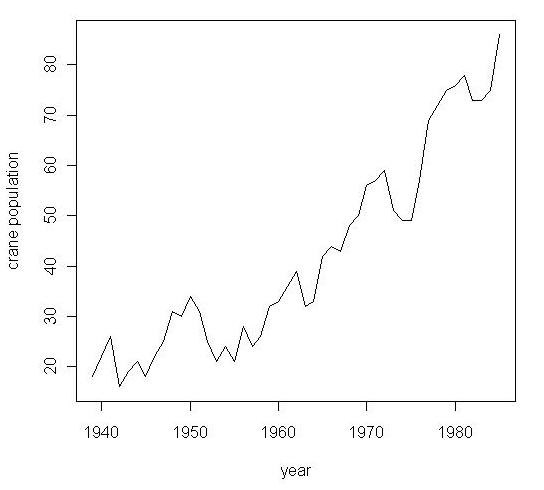
\includegraphics[width = .6\textwidth]{images/goose.png}
\end{center}

\end{frame}
